
\documentclass[tikz,border=1pt]{standalone}

\usepackage{amsmath}
\usepackage{xcolor}
\usepackage{tikz}
\usetikzlibrary{calc, fit, matrix, positioning}

\tikzstyle{circ}=[circle, draw, minimum size=1.2cm]
\tikzstyle{square}=[rectangle, draw, minimum size=1cm]

\begin{document}

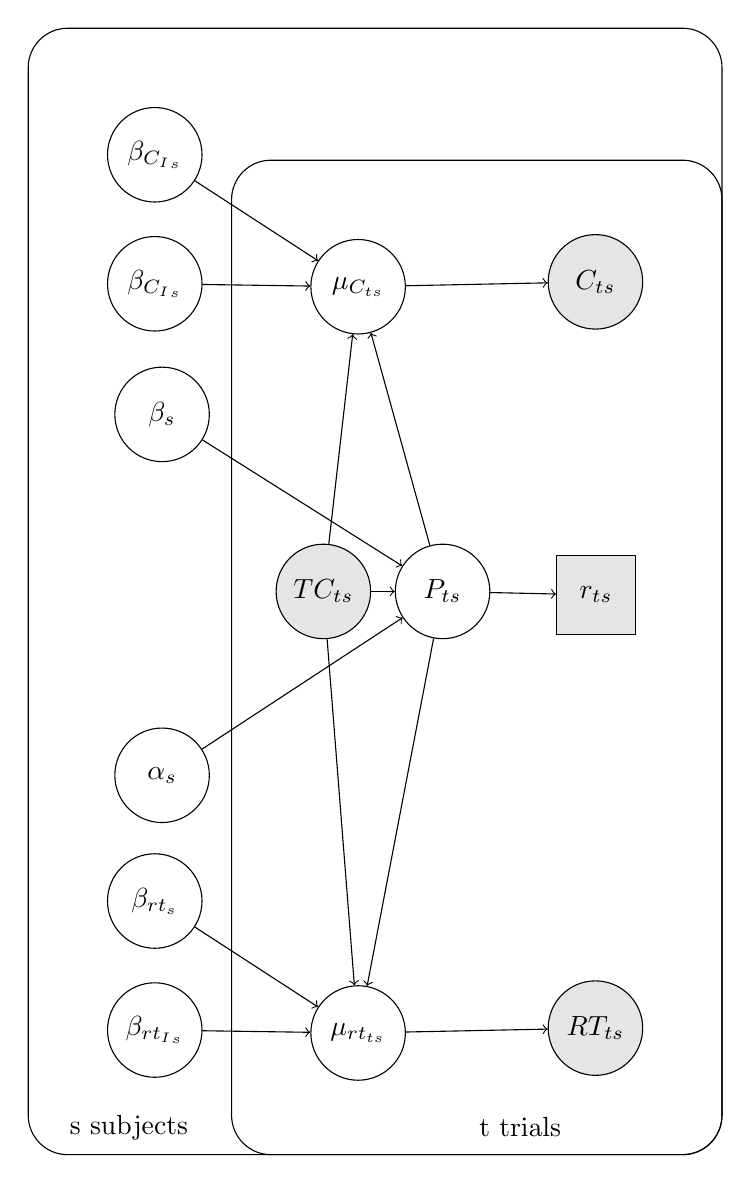
\begin{tikzpicture}

% Matrix m0
\matrix (m0) [
    ampersand replacement=\&,
    matrix of math nodes,
    nodes in empty cells,
    column sep=.3cm,
    row sep=0.4cm,
]
{
    \\
     |[circ, draw]| \beta_{{C_I}_{s}}\\
    |[circ, draw]| \beta_{{C_I}_{s}} \&\& \& |[circ, draw]| \mu_{{C}_{ts}} \& | [minimum size=1.2cm, inner sep=0pt, draw=none]|\& |[circ, draw, fill=gray!20]| C_{ts}\\
    \\   
};

\draw[->] (m0-2-1) to (m0-3-4);
\draw[->] (m0-3-1) to (m0-3-4);
\draw[->] (m0-3-4) to (m0-3-6);

% Matrix m1 (below m0)
\matrix (m1) [
    ampersand replacement=\&,
    matrix of math nodes,
    nodes in empty cells,
    column sep=.3cm,
    row sep=0.4cm,
    below=-0.5cm of m0
]
{
    |[circ, draw]| \beta_{s}\\
    \\
    | [minimum size=1.2cm, inner sep=0pt, draw=none]|\&\& |[circ, draw, fill=gray!20]| TC_{ts}\&  |[circ, draw]| P_{ts} \&\&  |[square, draw, fill=gray!20]| r_{ts}  \\
    \\
    |[circ, draw]| \alpha_{s} \\
};

\draw[->] (m1-1-1) to (m1-3-4);
\draw[->] (m1-5-1) to (m1-3-4);
\draw[->] (m1-3-4) to (m1-3-6);
\draw[->] (m1-3-3) to (m1-3-4);
\draw[->] (m1-3-4) to (m0-3-4);
\draw[->] (m1-3-3) to (m0-3-4);


% Matrix m2 (below m1)
\matrix (m2) [
    ampersand replacement=\&,
    matrix of math nodes,
    nodes in empty cells,
    column sep=.3cm,
    row sep=0.4cm,
    below=-0.5cm of m1
]
{
    \\
     |[circ, draw]| \beta_{{rt}_{s}}\\
    |[circ, draw]| \beta_{{rt_I}_{s}} \&\& \& |[circ, draw]| \mu_{{rt}_{ts}} \& | [minimum size=1.2cm, inner sep=0pt, draw=none]|\& |[circ, draw, fill=gray!20]| RT_{ts}\\
    \\
};

\draw[->] (m2-2-1) to (m2-3-4);
\draw[->] (m2-3-1) to (m2-3-4);
\draw[->] (m2-3-4) to (m2-3-6);
\draw[->] (m1-3-4) to (m2-3-4);
\draw[->] (m1-3-3) to (m2-3-4);
% Plates
\pgfsetcornersarced{\pgfpoint{5mm}{5mm}}
\node[draw=black, fit=(m0-2-1) (m2-3-6), inner sep=10mm] {};
\pgfsetcornersarced{\pgfpoint{5mm}{5mm}}
\node[draw=black, fit=(m0-3-4) (m2-3-6), inner sep=10mm] {};

\node[rotate=0, anchor=west] at (-4.0,-11.5) {s subjects};
\node[rotate=0, anchor=west] at (1.2,-11.5) {t trials};

\end{tikzpicture}


\end{document}
